\documentclass[10pt,aspectratio=169]{beamer}
\usepackage[T1]{fontenc}
\usepackage{lmodern}
\usepackage{booktabs}
\usepackage{tikz}
\definecolor{jhublue}{HTML}{173A63}
\definecolor{lora}{HTML}{147D78}
\definecolor{base}{HTML}{64748B}
\definecolor{lightline}{HTML}{D8E1E8}
\setbeamercolor{normal text}{fg=black,bg=white}
\setbeamercolor{frametitle}{fg=jhublue}
\setbeamerfont{frametitle}{size=\large,series=\bfseries}
\setbeamertemplate{navigation symbols}{}
\setbeamertemplate{footline}{\hfill\scriptsize Generalization: SQuAD 1.1 \quad \insertframenumber/3\hspace{0.6cm}\vspace{0.25cm}}
\setbeamersize{text margin left=0.7cm,text margin right=0.7cm}
\newcommand{\smallnote}[1]{{\scriptsize\color{base}#1}}
\begin{document}

\begin{frame}{Does LoRA resist irrelevant preceding text?}
\vspace{0.1cm}
{\large\bfseries Research question}\par\vspace{0.18cm}
Does a fine-tuned Qwen3-0.6B model lose less short-answer accuracy than its base model when unrelated text is placed before the answer passage?\par\vspace{0.38cm}
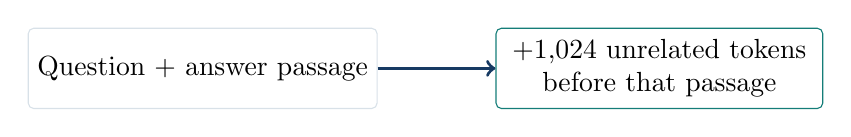
\begin{tikzpicture}[every node/.style={font=\normalsize}]
\node[draw=lightline,rounded corners=2pt,minimum width=3.8cm,minimum height=1.02cm,align=center] (q) at (2.1,0) {Question + answer passage};
\node[draw=lora,rounded corners=2pt,minimum width=4.15cm,minimum height=1.02cm,align=center] (d) at (7.9,0) {+1,024 unrelated tokens\\before that passage};
\draw[->,very thick,color=jhublue] (q.east)--(d.west);
\end{tikzpicture}
\vspace{0.35cm}
\begin{columns}[T,onlytextwidth]
\column{0.48\textwidth}
\textbf{Controls}\par
Same 900-question published SQuAD test list, prompt, checkpoint, greedy decoding, and 64-token cap. Two fixed distractor seeds.
\column{0.49\textwidth}
\textbf{Two stages}\par
Initial 90 questions; then the remaining 810, all from the same 45 articles. Pair models on each question; bootstrap articles.
\end{columns}
\vfill
\smallnote{Original prediction: LoRA EM would fall by at least 8 percentage points at +1,024 tokens. The first 90-question point estimate did not meet it.}
\end{frame}

\begin{frame}{Initial 90 questions: the predicted 8-point drop was not observed}
\centering
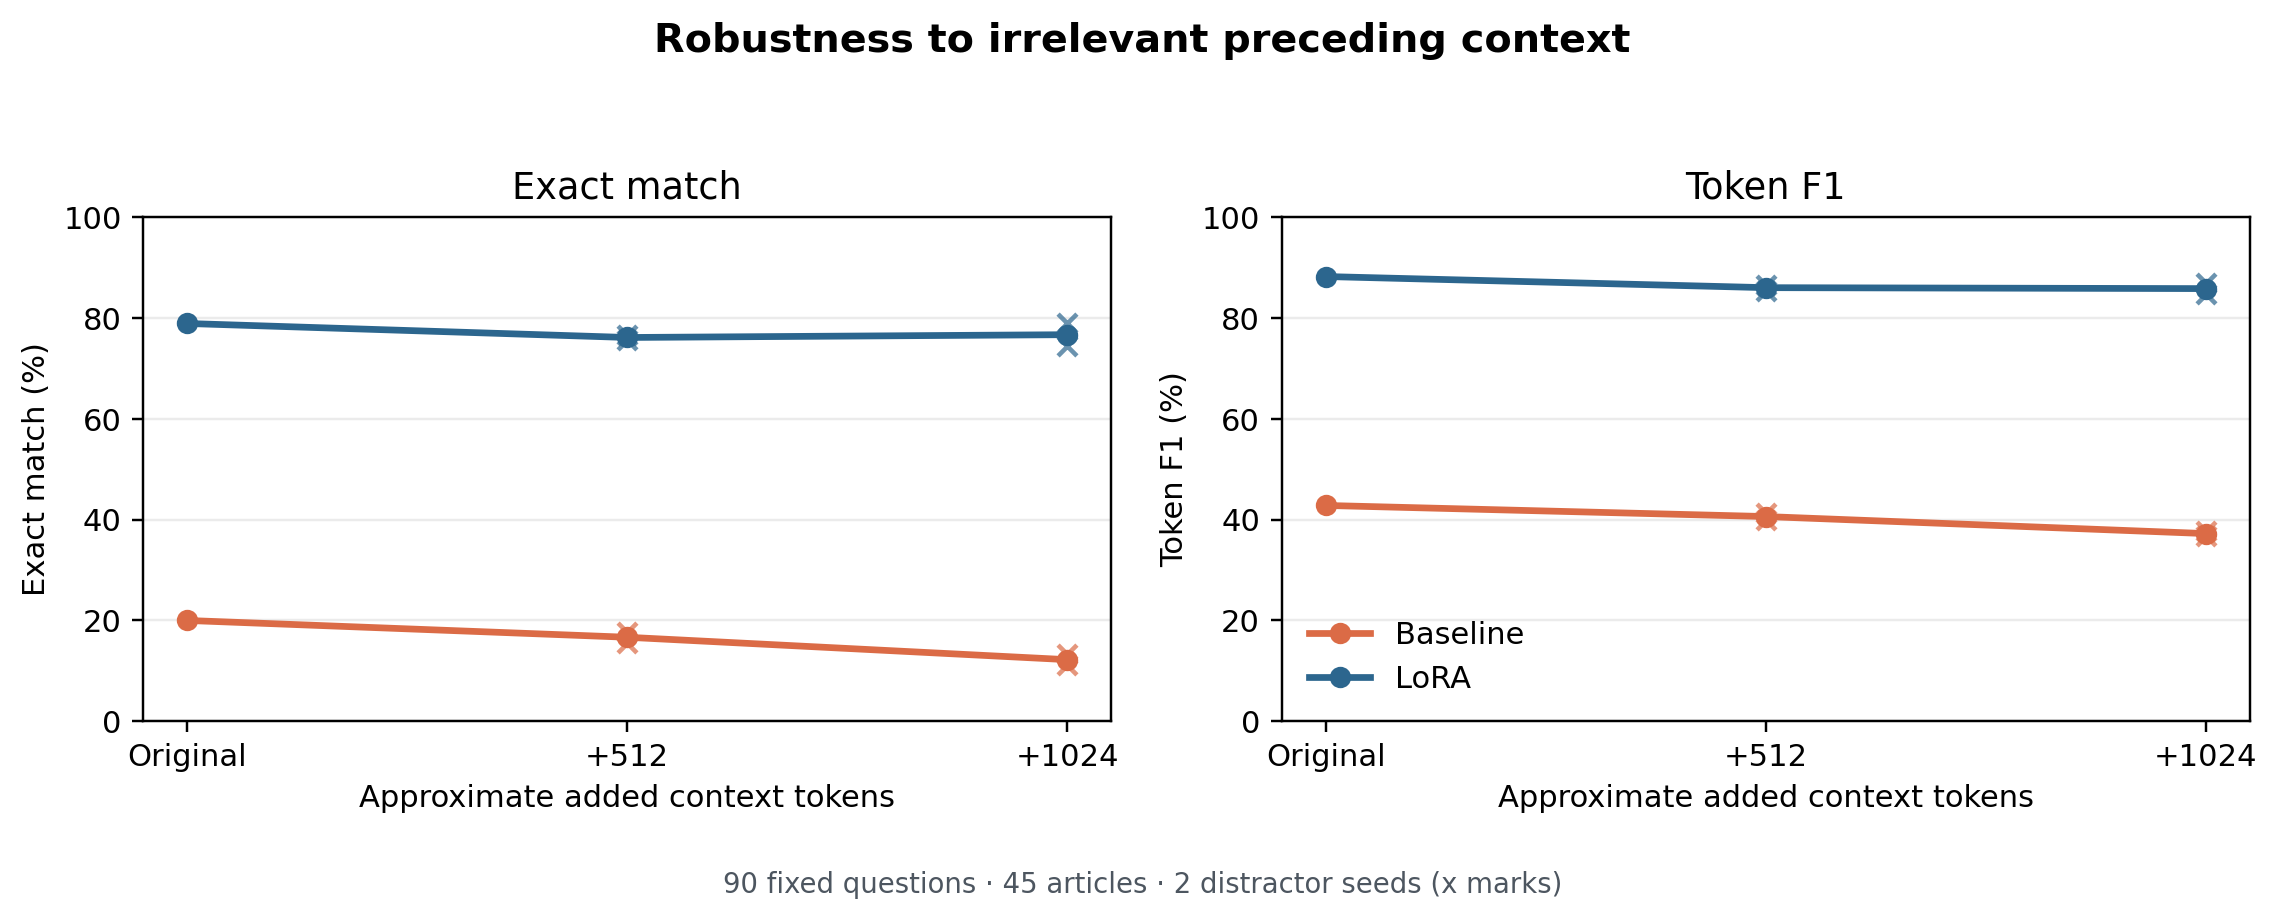
\includegraphics[width=\textwidth,height=5.65cm,keepaspectratio]{figures/initial_90_length_effects.png}
\vspace{0.12cm}
\parbox{\textwidth}{\small LoRA EM changed by \textbf{--2.22 pp} at +1,024 tokens (95\% article-bootstrap CI \textbf{--8.89 to +3.89}). The direct LoRA--Base contrast was +5.56 pp (CI --3.89 to +15.56): inconclusive.}
\end{frame}

\begin{frame}{Follow-up 810 questions: LoRA's EM drop was smaller}
\centering
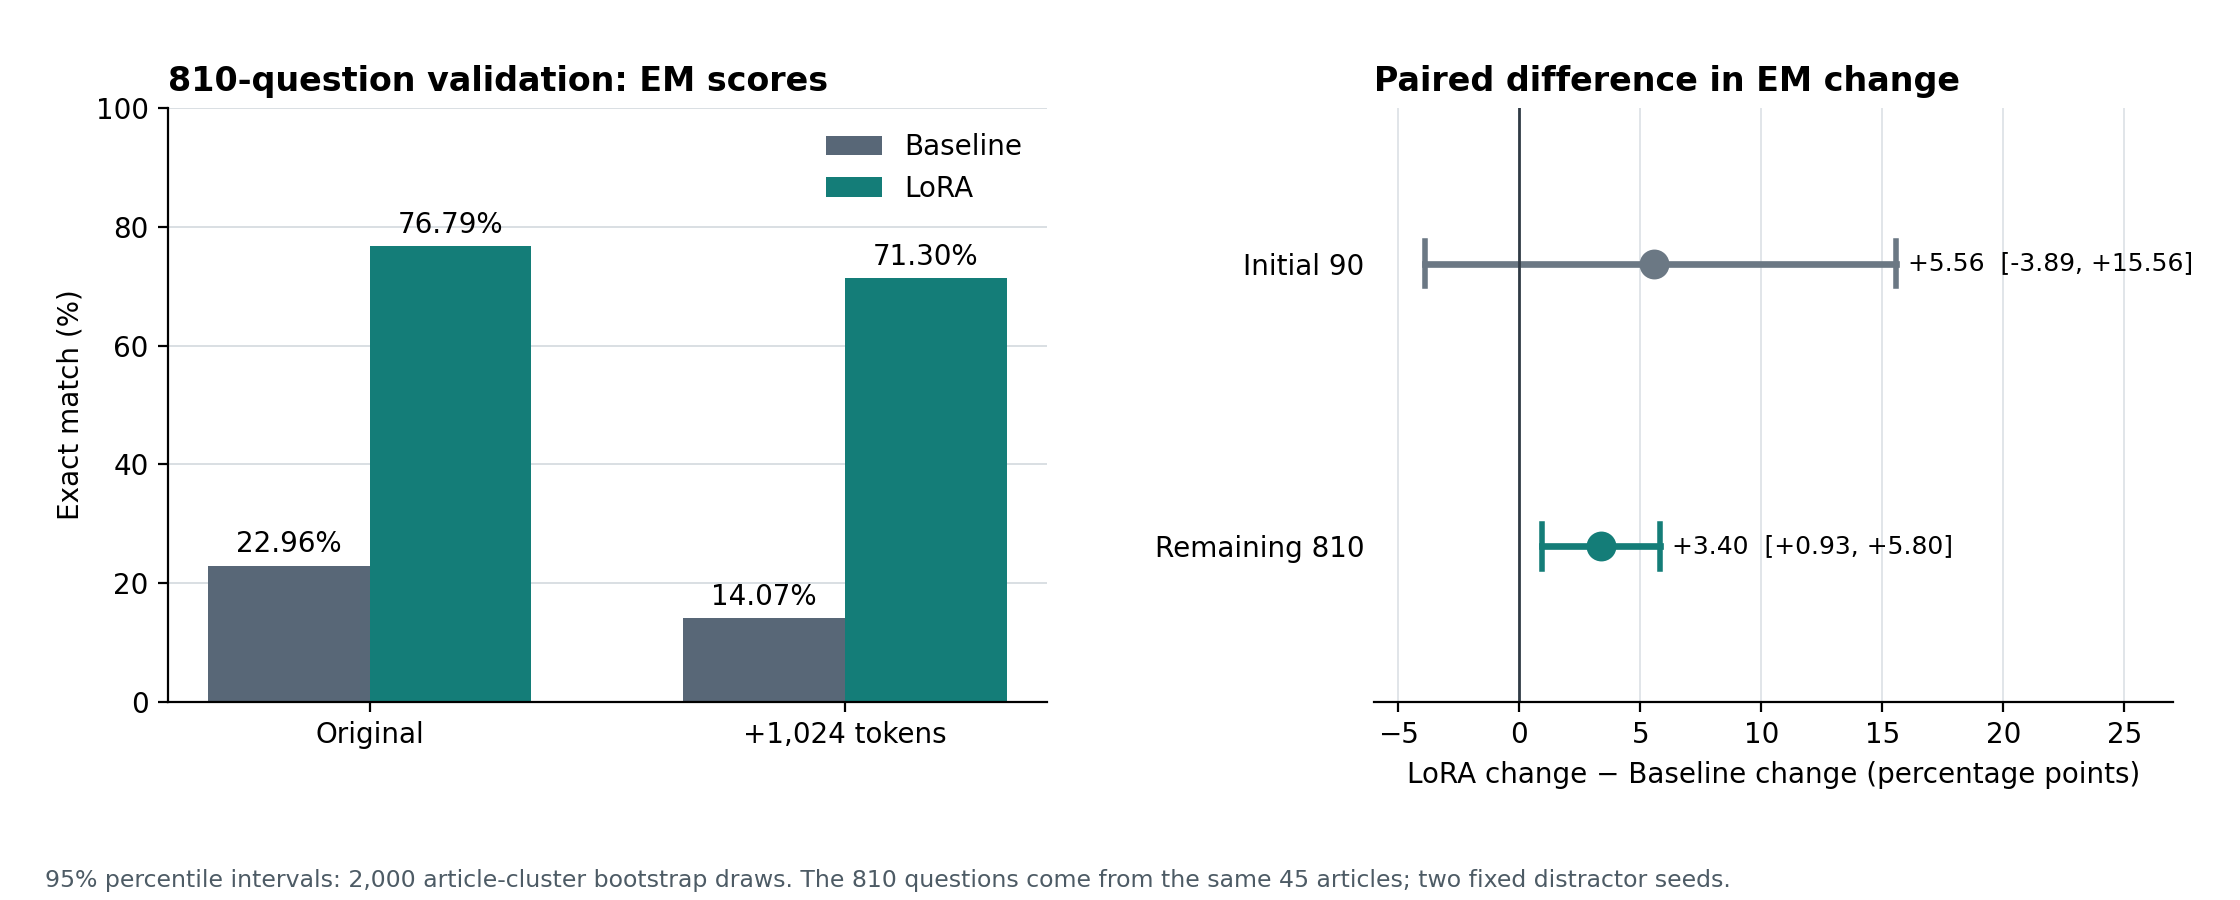
\includegraphics[width=\textwidth,height=5.65cm,keepaspectratio]{figures/validation_810_quantitative.png}
\vspace{0.12cm}
\parbox{\textwidth}{\small \textbf{Direct paired effect: +3.40 pp} (95\% article-bootstrap CI \textbf{+0.93 to +5.80}). Same 45 articles, two fixed distractor seeds, one LoRA checkpoint. Error audit: 138/149 wrong strings were found only in the original passage.}
\end{frame}
\end{document}
